\documentclass[a4paper,11pt]{article}\usepackage[]{graphicx}\usepackage[]{color}
%% maxwidth is the original width if it is less than linewidth
%% otherwise use linewidth (to make sure the graphics do not exceed the margin)
\makeatletter
\def\maxwidth{ %
  \ifdim\Gin@nat@width>\linewidth
    \linewidth
  \else
    \Gin@nat@width
  \fi
}
\makeatother

\definecolor{fgcolor}{rgb}{0.345, 0.345, 0.345}
\newcommand{\hlnum}[1]{\textcolor[rgb]{0.686,0.059,0.569}{#1}}%
\newcommand{\hlstr}[1]{\textcolor[rgb]{0.192,0.494,0.8}{#1}}%
\newcommand{\hlcom}[1]{\textcolor[rgb]{0.678,0.584,0.686}{\textit{#1}}}%
\newcommand{\hlopt}[1]{\textcolor[rgb]{0,0,0}{#1}}%
\newcommand{\hlstd}[1]{\textcolor[rgb]{0.345,0.345,0.345}{#1}}%
\newcommand{\hlkwa}[1]{\textcolor[rgb]{0.161,0.373,0.58}{\textbf{#1}}}%
\newcommand{\hlkwb}[1]{\textcolor[rgb]{0.69,0.353,0.396}{#1}}%
\newcommand{\hlkwc}[1]{\textcolor[rgb]{0.333,0.667,0.333}{#1}}%
\newcommand{\hlkwd}[1]{\textcolor[rgb]{0.737,0.353,0.396}{\textbf{#1}}}%

\usepackage{framed}
\makeatletter
\newenvironment{kframe}{%
 \def\at@end@of@kframe{}%
 \ifinner\ifhmode%
  \def\at@end@of@kframe{\end{minipage}}%
  \begin{minipage}{\columnwidth}%
 \fi\fi%
 \def\FrameCommand##1{\hskip\@totalleftmargin \hskip-\fboxsep
 \colorbox{shadecolor}{##1}\hskip-\fboxsep
     % There is no \\@totalrightmargin, so:
     \hskip-\linewidth \hskip-\@totalleftmargin \hskip\columnwidth}%
 \MakeFramed {\advance\hsize-\width
   \@totalleftmargin\z@ \linewidth\hsize
   \@setminipage}}%
 {\par\unskip\endMakeFramed%
 \at@end@of@kframe}
\makeatother

\definecolor{shadecolor}{rgb}{.97, .97, .97}
\definecolor{messagecolor}{rgb}{0, 0, 0}
\definecolor{warningcolor}{rgb}{1, 0, 1}
\definecolor{errorcolor}{rgb}{1, 0, 0}
\newenvironment{knitrout}{}{} % an empty environment to be redefined in TeX

\usepackage{alltt}

\usepackage{amsmath}
\usepackage{times}
\usepackage{hyperref}
\usepackage[numbers, round]{natbib}
\usepackage[american]{babel}
\usepackage{authblk}
\usepackage{subfig}
\usepackage{placeins}
\usepackage{footnote}
\usepackage{tabularx}
\usepackage{parskip}
\usepackage{threeparttable}

\usepackage{longtable}

\renewcommand\Affilfont{\itshape\small}

\usepackage{csquotes}
\usepackage{setspace}

\doublespacing

\renewcommand{\topfraction}{0.85}
\renewcommand{\textfraction}{0.1}
\usepackage{graphicx}


\usepackage{mathptmx}% Times Roman font
\usepackage[scaled=.90]{helvet}% Helvetica, served as a model for arial

\usepackage{indentfirst}
\setlength{\parskip}{0pt}

\usepackage{courier}

\usepackage{titlesec}
\usepackage{titletoc}

\titleformat{\section}
  {\normalfont\sffamily\bfseries\LARGE}
  {\thesection}{0.5em}{}
\titleformat{\subsection}
  {\normalfont\sffamily\bfseries\Large}
  {\thesubsection}{0.5em}{}
\titleformat{\subsubsection}
  {\normalfont\sffamily\large}
  {\thesubsubsection}{0.5em}{}
  
\titlecontents{section}
[2em]                 % adjust left margin
{\sffamily}             % font formatting
{\contentslabel{2.3em}} % section label and offset
{\hspace*{-2.3em}}
{\titlerule*[0.25pc]{.}\contentspage}
  
\titlecontents{subsection}
[4.6em]                 % adjust left margin
{\sffamily}             % font formatting
{\contentslabel{2.3em}} % section label and offset
{\hspace*{-2.3em}}
{\titlerule*[0.25pc]{.}\contentspage}
  
\titlecontents{subsubsection}
[6.9em]                 % adjust left margin
{\sffamily}             % font formatting
{\contentslabel{2.3em}} % section label and offset
{\hspace*{-2.3em}}
{\titlerule*[0.25pc]{.}\contentspage}

\titlecontents{table}
[0em]                 % adjust left margin
{\sffamily}             % font formatting
{\textbf{Table}\hspace*{2em} \contentslabel {2em}} % section label and offset
{\hspace*{4em}}
{\titlerule*[0.25pc]{.}\contentspage}

\titlecontents{figure}
[0em]                 % adjust left margin
{\sffamily}             % font formatting
{\textbf{Figure}\hspace*{2em} \contentslabel {2em}} % section label and offset
{\hspace*{4em}}
{\titlerule*[0.25pc]{.}\contentspage}

%Italisize and change font of urls:
\urlstyle{sf}
\renewcommand\UrlFont\itshape

\usepackage{caption}
\captionsetup{
  font={sf},
  labelfont={bf,sf},
  labelsep=period,
  justification=justified,
  singlelinecheck=false
}

\setlength\parindent{20pt}

\textwidth=6.5in
\textheight=9.2in
\parskip=.3cm
\oddsidemargin=.1in
\evensidemargin=.1in
\headheight=-.3in

%------------------------------------------------------------
% newcommand
%------------------------------------------------------------
\newcommand{\scscst}{\scriptscriptstyle}
\newcommand{\scst}{\scriptstyle}
\newcommand{\Robject}[1]{{\texttt{#1}}}
\newcommand{\Rfunction}[1]{{\texttt{#1}}}
\newcommand{\Rclass}[1]{\textit{#1}}
\newcommand{\Rpackage}[1]{\textit{#1}}
\newcommand{\Rexpression}[1]{\texttt{#1}}
\newcommand{\Rmethod}[1]{{\texttt{#1}}}
\newcommand{\Rfunarg}[1]{{\texttt{#1}}}
\IfFileExists{upquote.sty}{\usepackage{upquote}}{}
\begin{document}

\renewenvironment{knitrout}{\begin{singlespace}}{\end{singlespace}}
\renewcommand*\listfigurename{Figures}
\renewcommand*\listtablename{Tables}






%------------------------------------------------------------
\title{Search Test}
%------------------------------------------------------------
\author[1]{Laura De Cicco}
\affil[1]{United States Geological Survey}

% \maketitle

\noindent{\huge\textsf{\textbf{Search Test}}}

\noindent\textsf{\today}
% 
% \tableofcontents
% \listoffigures
% \listoftables

%------------------------------------------------------------ 
\section{Load Data}
\label{sec:load}
%------------------------------------------------------------

The following code is used to pull raw data from the Water Quality Portal \url{http://www.waterqualitydata.us/}. The user is responsible for choosing a parameter and huc.

\begin{knitrout}
\definecolor{shadecolor}{rgb}{0.969, 0.969, 0.969}\color{fgcolor}\begin{kframe}
\begin{alltt}
\hlkwd{library}\hlstd{(dataRetrieval)}
\hlkwd{library}\hlstd{(dplyr)}
\hlkwd{library}\hlstd{(USGSHydroTools)}


\hlstd{data} \hlkwb{<-} \hlkwd{readWQPdata}\hlstd{(}\hlkwc{huc}\hlstd{=}\hlstr{"0207*"}\hlstd{,} \hlkwc{characteristicName}\hlstd{=}\hlstr{"Phosphorus"}\hlstd{)}
\hlcom{#data <- readWQPdata(huc="0410*", characteristicName="Phosphorus")}
\hlstd{sites} \hlkwb{<-}  \hlkwd{whatWQPsites}\hlstd{(}\hlkwc{huc}\hlstd{=}\hlstr{"0207*"}\hlstd{,} \hlkwc{characteristicName}\hlstd{=}\hlstr{"Phosphorus"}\hlstd{)}
\hlcom{#sites <-  whatWQPsites(huc="0410*", characteristicName="Phosphorus")}

\hlstd{data_bySite} \hlkwb{<-} \hlkwd{group_by}\hlstd{(data, MonitoringLocationIdentifier)}
\hlstd{summarize} \hlkwb{<-}  \hlkwd{summarise}\hlstd{(data_bySite,}
  \hlkwc{Count} \hlstd{=} \hlkwd{n}\hlstd{(),}
  \hlkwc{CountAfter2000} \hlstd{=} \hlkwd{sum}\hlstd{(ActivityStartDateTime} \hlopt{>}
                     \hlkwd{as.POSIXct}\hlstd{(}\hlstr{"2000-01-01 00:00:00"}\hlstd{),}\hlkwc{na.rm} \hlstd{=} \hlnum{TRUE}\hlstd{),}
  \hlkwc{MinDate} \hlstd{=} \hlkwd{min}\hlstd{(ActivityStartDateTime,} \hlkwc{na.rm} \hlstd{=} \hlnum{TRUE}\hlstd{),}
  \hlkwc{MaxDate} \hlstd{=} \hlkwd{max}\hlstd{(ActivityStartDateTime,} \hlkwc{na.rm} \hlstd{=} \hlnum{TRUE}\hlstd{))} \hlopt
  \hlkwd{arrange}\hlstd{(}\hlkwd{desc}\hlstd{(Count))}  \hlopt
  \hlkwd{filter}\hlstd{(Count} \hlopt{>=} \hlnum{50}\hlstd{)} \hlopt
  \hlkwd{filter}\hlstd{(CountAfter2000} \hlopt{>=} \hlnum{10}\hlstd{)}
\end{alltt}
\end{kframe}
\end{knitrout}


% latex table generated in R 3.1.1 by xtable 1.7-4 package
% Wed Feb 18 11:43:45 2015
\begin{table}[ht]
\centering
\begin{tabular}{rlrrll}
  \hline
 & MonitoringLocationIdentifier & Count & CountAfter2000 & MinDate & MaxDate \\ 
  \hline
1 & MDDNR-LE2.2 & 1887 &  21 & 1984-08-06 & 2007-10-01 \\ 
  2 & MDDNR-TF2.4 & 1710 &  17 & 1986-01-06 & 2007-10-02 \\ 
  3 & MDDNR-RET2.2 & 1678 &  17 & 1984-07-19 & 2007-10-02 \\ 
  4 & MDDNR-RET2.4 & 1602 &  13 & 1986-01-06 & 2007-10-05 \\ 
  5 & MDDNR-LE2.3 & 1599 & 497 & 1984-07-11 & 2013-12-10 \\ 
  6 & USGS-01646580 & 1393 & 664 & 1973-02-05 & 2015-01-08 \\ 
  7 & MDDNR-TF2.3 & 1392 &  12 & 1984-07-19 & 2000-04-24 \\ 
  8 & MDDNR-TF2.2 & 1302 &  12 & 1986-01-06 & 2000-04-24 \\ 
  9 & USGS-01614500 & 1287 & 447 & 1973-09-12 & 2004-09-20 \\ 
  10 & USGS-01645762 & 906 & 906 & 2008-04-24 & 2014-12-09 \\ 
  11 & USGS-01646305 & 902 & 902 & 2008-04-24 & 2014-12-09 \\ 
  12 & USGS-01658000 & 888 & 888 & 2000-10-24 & 2015-01-13 \\ 
  13 & USGS-01645704 & 851 & 851 & 2008-04-24 & 2014-12-09 \\ 
  14 & USGS-01656903 & 832 & 832 & 2008-04-24 & 2014-12-09 \\ 
  15 & USGS-01648010 & 498 & 496 & 1999-06-25 & 2014-12-18 \\ 
  16 & USGS-01634000 & 471 & 293 & 1976-08-31 & 2014-12-17 \\ 
  17 & USGS-01631000 & 469 & 295 & 1994-06-08 & 2014-12-17 \\ 
  18 & USGS-01658500 & 458 & 345 & 1994-08-23 & 2014-12-11 \\ 
  19 & USGS-01649500 & 432 & 421 & 1969-10-23 & 2014-12-03 \\ 
  20 & USGS-01649190 & 425 & 425 & 2007-07-23 & 2015-01-07 \\ 
  21 & MDDNR-NBP0689 & 354 &  82 & 1986-01-09 & 2004-02-11 \\ 
  22 & MDDNR-NBP0534 & 352 &  78 & 1986-01-09 & 2004-02-10 \\ 
  23 & MDDNR-SAV0000 & 337 &  71 & 1986-01-09 & 2004-02-10 \\ 
  24 & MDDNR-TOW0030 & 329 &  60 & 1986-02-06 & 2004-02-12 \\ 
  25 & MDDNR-POT1830 & 324 &  49 & 1986-01-30 & 2004-02-12 \\ 
  26 & MDDNR-SEN0008 & 324 &  49 & 1986-01-08 & 2004-02-11 \\ 
  27 & MDDNR-BPC0035 & 323 &  49 & 1986-01-27 & 2004-02-12 \\ 
  28 & MDDNR-CAC0031 & 323 &  49 & 1986-01-28 & 2004-02-12 \\ 
  29 & MDDNR-MON0155 & 323 &  49 & 1986-01-27 & 2004-02-12 \\ 
  30 & MDDNR-MON0269 & 323 &  49 & 1986-01-28 & 2004-02-12 \\ 
  31 & MDDNR-POT1471 & 323 &  49 & 1986-01-08 & 2004-02-12 \\ 
  32 & MDDNR-ANT0044 & 322 &  48 & 1986-01-30 & 2004-02-12 \\ 
  33 & MDDNR-POT1595 & 322 &  49 & 1986-01-08 & 2004-02-12 \\ 
  34 & MDDNR-CAC0148 & 321 &  48 & 1986-01-28 & 2004-02-12 \\ 
  35 & MDDNR-GEO0009 & 321 &  50 & 1986-01-09 & 2004-02-10 \\ 
  36 & MDDNR-MON0020 & 321 &  48 & 1986-01-08 & 2004-02-12 \\ 
  37 & MDDNR-MON0528 & 321 &  49 & 1986-01-28 & 2004-02-12 \\ 
  38 & MDDNR-NBP0103 & 321 &  50 & 1986-01-10 & 2004-02-12 \\ 
  39 & MDDNR-ANT0203 & 320 &  49 & 1986-01-30 & 2004-02-10 \\ 
  40 & MDDNR-NBP0326 & 320 &  49 & 1986-01-08 & 2004-02-12 \\ 
  41 & MDDNR-POT2386 & 320 &  50 & 1986-01-30 & 2004-02-10 \\ 
  42 & MDDNR-ANA0082 & 319 &  49 & 1986-01-07 & 2004-02-11 \\ 
  43 & MDDNR-CON0005 & 319 &  49 & 1986-02-19 & 2004-02-10 \\ 
  44 & MDDNR-WIL0013 & 319 &  62 & 1986-01-09 & 2004-02-12 \\ 
  45 & USGS-01618000 & 319 &  88 & 1979-03-29 & 2002-08-05 \\ 
  46 & MDDNR-CON0180 & 318 &  49 & 1986-01-29 & 2004-02-10 \\ 
  47 & MDDNR-POT1596 & 317 &  48 & 1986-01-08 & 2004-02-12 \\ 
  48 & MDDNR-POT1184 & 316 &  48 & 1986-01-07 & 2004-02-11 \\ 
  49 & MDDNR-ANT0366 & 314 &  49 & 1986-01-29 & 2004-02-10 \\ 
  50 & MDDNR-CJB0005 & 314 &  52 & 1986-01-07 & 2004-02-11 \\ 
  51 & MDDNR-NBP0023 & 314 &  49 & 1986-01-10 & 2004-02-12 \\ 
  52 & MDDNR-RCM0111 & 314 &  49 & 1986-02-04 & 2004-02-11 \\ 
  53 & MDDNR-BDK0000 & 312 &  56 & 1986-01-09 & 2004-02-12 \\ 
  54 & MDDNR-POT1472 & 312 &  49 & 1986-02-03 & 2004-02-12 \\ 
  55 & MDDNR-NBP0461 & 302 &  45 & 1986-01-09 & 2004-02-12 \\ 
  56 & MDDNR-POT2766 & 296 &  43 & 1986-01-10 & 2004-02-12 \\ 
  57 & USGS-01636500 & 282 &  80 & 1972-05-17 & 2014-12-18 \\ 
  58 & USGS-01621050 & 277 & 110 & 1993-03-29 & 2014-12-17 \\ 
  59 & USGS-01611500 & 262 & 262 & 2000-10-24 & 2015-01-13 \\ 
  60 & USGS-01645940 & 257 & 257 & 2008-04-24 & 2014-12-09 \\ 
  61 & USGS-01645745 & 253 & 253 & 2008-04-24 & 2014-12-09 \\ 
  62 & USGS-01645844 & 253 & 253 & 2008-04-24 & 2014-12-09 \\ 
  63 & USGS-01654500 & 253 & 253 & 2012-10-09 & 2014-12-09 \\ 
  64 & USGS-01652860 & 243 & 243 & 2008-04-24 & 2014-12-09 \\ 
  65 & USGS-01653717 & 243 & 243 & 2008-04-24 & 2014-12-09 \\ 
  66 & USGS-0165690673 & 243 & 243 & 2008-04-24 & 2014-12-09 \\ 
  67 & USGS-01657322 & 243 & 243 & 2008-04-24 & 2014-12-09 \\ 
  68 & USGS-01657394 & 243 & 243 & 2008-04-24 & 2014-12-09 \\ 
  69 & USGS-01652789 & 242 & 242 & 2008-04-24 & 2014-12-09 \\ 
  70 & USGS-0165694286 & 240 & 240 & 2008-04-24 & 2014-12-09 \\ 
  71 & 21PA\_WQX-WQN0501 & 233 & 225 & 1998-10-14 & 2014-09-17 \\ 
  72 & USGS-01654000 & 219 &  82 & 1993-04-20 & 2014-12-11 \\ 
  73 & USGS-01659000 & 210 & 209 & 1994-08-23 & 2011-09-20 \\ 
  74 & USGS-01608500 & 208 & 191 & 1972-05-18 & 2015-01-13 \\ 
  75 & USGS-01651000 & 207 & 196 & 1969-10-23 & 2010-06-09 \\ 
  76 & 21PA\_WQX-WQN0509 & 196 & 196 & 2010-10-05 & 2014-09-17 \\ 
  77 & USGS-01604500 & 195 & 195 & 2005-06-07 & 2015-01-12 \\ 
  78 & 21PA\_WQX-WQN0511 & 190 & 190 & 2010-10-06 & 2014-09-17 \\ 
  79 & USGS-01616500 & 185 & 185 & 2005-06-09 & 2015-01-14 \\ 
  80 & 21PA\_WQX-WQN0510 & 181 & 181 & 2010-10-13 & 2014-09-10 \\ 
  81 & 21PA\_WQX-WQN0512 & 172 & 172 & 2010-10-14 & 2014-09-10 \\ 
  82 & USGS-01653600 & 168 & 168 & 2000-10-24 & 2002-10-18 \\ 
  83 & USGS-01650800 & 165 & 165 & 2012-07-19 & 2015-01-14 \\ 
  84 & 21PA\_WQX-WQN0513 & 156 & 156 & 2010-10-04 & 2014-09-10 \\ 
  85 & USGS-01632900 & 154 & 154 & 2010-04-15 & 2014-12-17 \\ 
  86 & USGS-01660110 & 150 &  48 & 1996-02-07 & 2001-12-12 \\ 
  87 & USGS-01646000 & 142 & 142 & 2011-07-13 & 2014-12-11 \\ 
  88 & USGS-01610155 & 120 & 116 & 1985-08-28 & 2002-08-05 \\ 
  89 & USGS-01661050 & 118 & 115 & 1992-06-01 & 2002-09-03 \\ 
  90 & USGS-01660500 & 100 &  24 & 1997-03-18 & 2000-12-19 \\ 
  91 & USGS-01651770 &  92 &  92 & 2012-10-02 & 2014-12-23 \\ 
  92 & USGS-01651800 &  92 &  92 & 2012-08-08 & 2014-12-24 \\ 
  93 & USGS-01618100 &  88 &  88 & 2011-06-14 & 2015-01-14 \\ 
  94 & USGS-01613030 &  87 &  87 & 2011-07-12 & 2015-01-14 \\ 
  95 & USGS-01595300 &  82 &  82 & 2012-06-11 & 2015-01-12 \\ 
  96 & USGS-01621410 &  82 &  82 & 2000-10-12 & 2001-09-06 \\ 
  97 & USGS-0164425950 &  81 &  81 & 2012-10-09 & 2014-12-09 \\ 
  98 & USGS-01644343 &  81 &  81 & 2012-10-09 & 2014-12-09 \\ 
  99 & USGS-01653844 &  81 &  81 & 2012-10-09 & 2014-12-09 \\ 
  100 & USGS-01655305 &  81 &  81 & 2012-10-09 & 2014-12-09 \\ 
  101 & USGS-01657100 &  81 &  81 & 2012-10-09 & 2014-12-09 \\ 
  102 & USGS-01614000 &  80 &  80 & 2012-06-13 & 2015-01-14 \\ 
  103 & USGS-01616400 &  79 &  79 & 2011-07-13 & 2014-12-18 \\ 
  104 & USGS-01642438 &  75 &  75 & 2008-08-25 & 2010-12-02 \\ 
  105 & USGS-01658705 &  74 &  54 & 1999-04-08 & 2001-06-11 \\ 
  106 & USGS-01658698 &  72 &  52 & 1999-04-08 & 2001-06-11 \\ 
  107 & USGS-01660920 &  58 &  58 & 2000-09-27 & 2002-06-19 \\ 
  108 & USGS-01615000 &  54 &  45 & 1969-11-20 & 2009-05-06 \\ 
  109 & USGS-01646500 &  53 &  50 & 1983-04-20 & 2014-08-29 \\ 
  110 & 21PA\_WQX-WQN0514 &  52 &  52 & 2010-10-27 & 2014-09-22 \\ 
   \hline
\end{tabular}
\caption{Sites with counts at least 50 samples and at least 10 after 2000} 
\label{tab:Summary}
\end{table}




\begin{knitrout}
\definecolor{shadecolor}{rgb}{0.969, 0.969, 0.969}\color{fgcolor}\begin{figure}
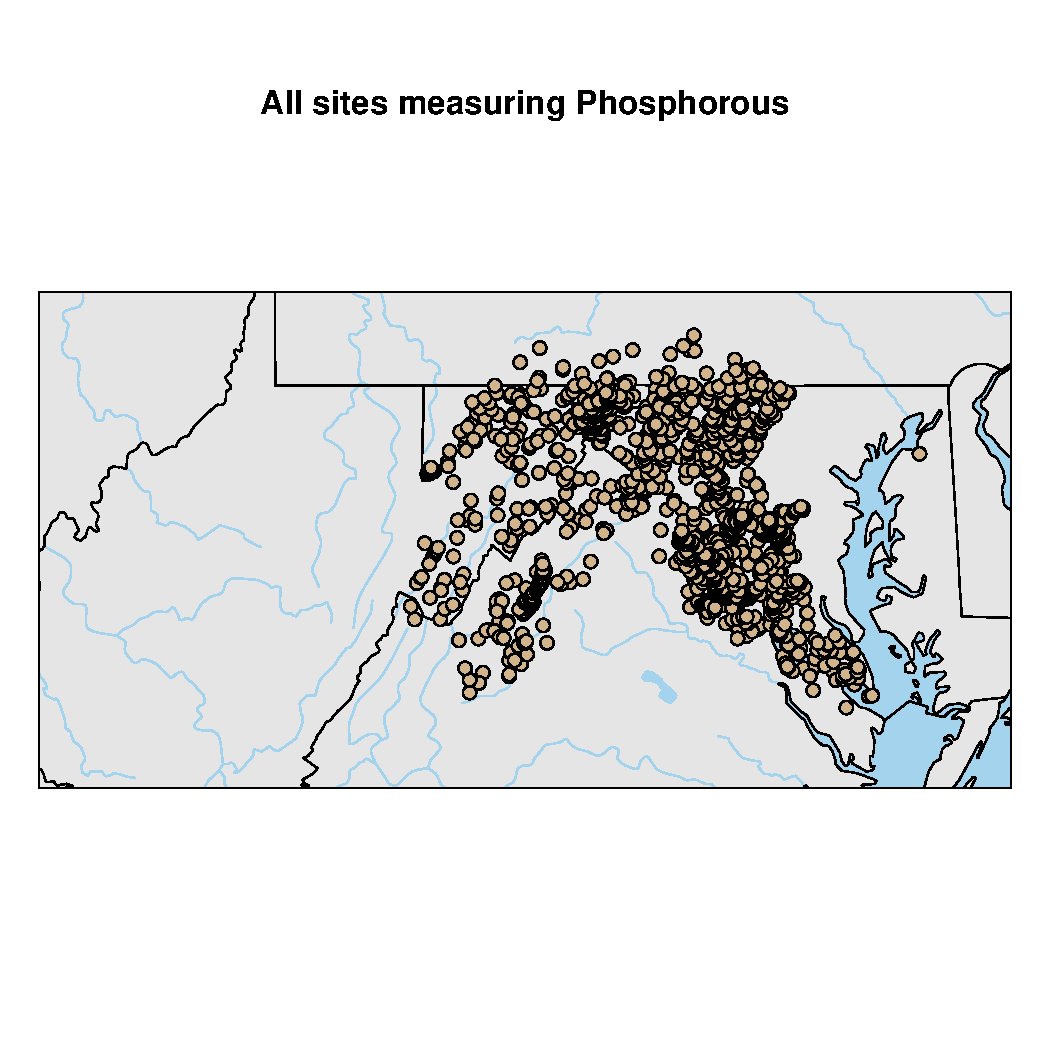
\includegraphics[width=\maxwidth]{figure/plotMap-1} \caption[Map of all sites]{Map of all sites}\label{fig:plotMap}
\end{figure}


\end{knitrout}


\begin{knitrout}
\definecolor{shadecolor}{rgb}{0.969, 0.969, 0.969}\color{fgcolor}\begin{figure}
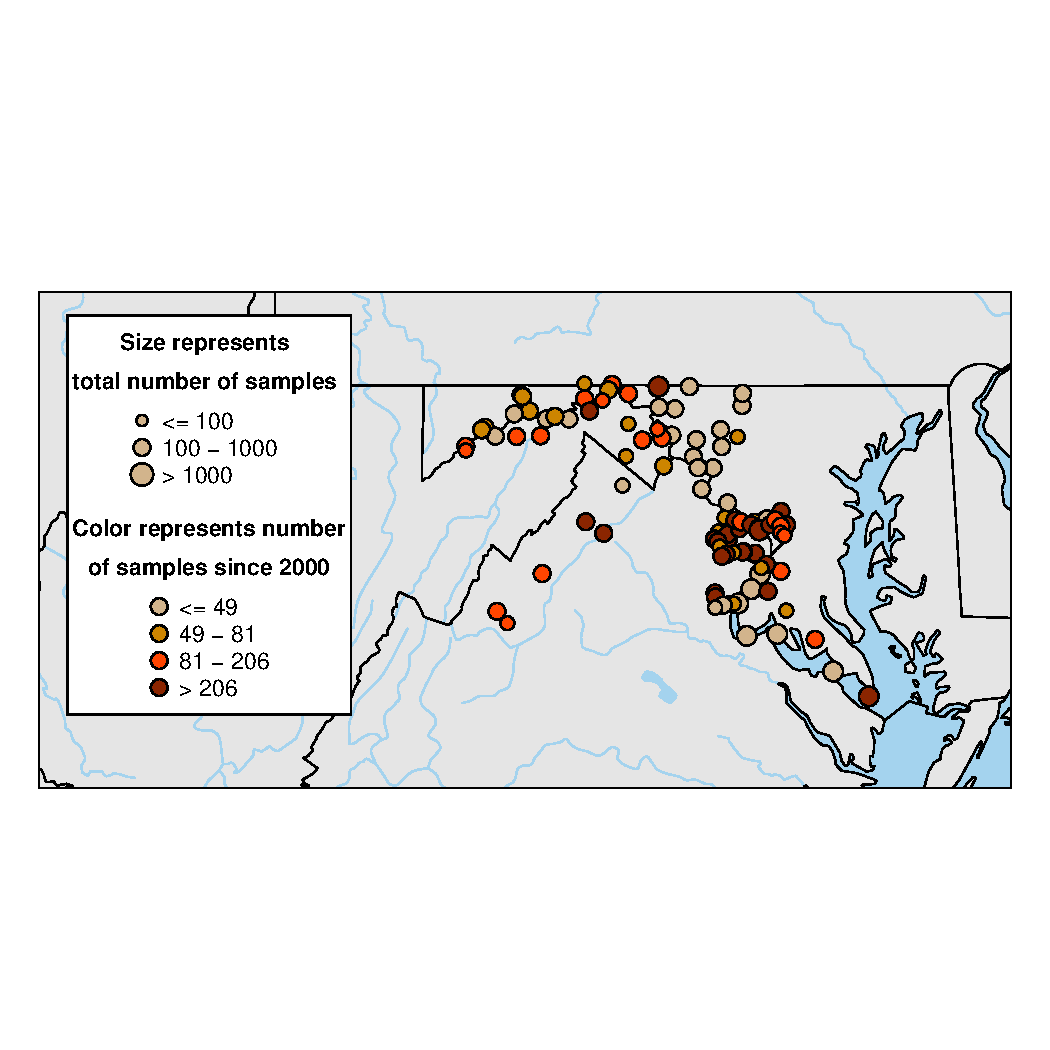
\includegraphics[width=\maxwidth]{figure/filteredMap-1} \caption[Map of sites with at least 50 samples and 10 since 2000]{Map of sites with at least 50 samples and 10 since 2000}\label{fig:filteredMap}
\end{figure}


\end{knitrout}

% # <<getDischarge>>=
% # 
% # siteIDs <- sapply(strsplit(sumStation$MonitoringLocationIdentifier, "-"), function(x) x[2])
% # sumStation$siteIDs <- siteIDs
% # 
% # dataAvail <- getNWISDataAvailability(siteIDs,type = "dv")
% # dischargeAvailable <- filter(dataAvail, parameter_cd == "00060") %.%
% #   select(site_no, Qstart=startDate, Qend=endDate, Qcount=count)
% # 
% # mergedInfo <- merge(sumStation,dischargeAvailable, by.x="siteIDs", by.y="site_no")
% # mergedInfo <- select(mergedInfo, siteIDs, Count, CountAfter2000, 
% #                      MinDate, MaxDate, Qstart, Qend, Qcount, 
% #                      LatitudeMeasure, LongitudeMeasure)
% # mergedInfo$MinDate <- as.Date(mergedInfo$MinDate)
% # mergedInfo$MaxDate <- as.Date(mergedInfo$MaxDate)
% # @
% # 

\end{document}
